\documentclass[12pt,a4paper]{article}
\usepackage[utf8]{inputenc}
\usepackage[T1]{fontenc}
\usepackage{graphicx}
\usepackage{listings}
\usepackage{xcolor}
\usepackage{geometry}
\usepackage{hyperref}
\usepackage{float}
\usepackage{caption}
\usepackage{tikz}
\usetikzlibrary{shapes.geometric, arrows.meta, positioning, shadows, fit, calc}

\geometry{margin=1in}

% Code listing style
\lstdefinestyle{pythoncode}{
    language=Python,
    basicstyle=\ttfamily\small,
    keywordstyle=\color{blue}\bfseries,
    commentstyle=\color{green!60!black}\itshape,
    stringstyle=\color{red},
    showstringspaces=false,
    numbers=left,
    numberstyle=\tiny\color{gray},
    stepnumber=1,
    numbersep=8pt,
    backgroundcolor=\color{gray!10},
    frame=single,
    breaklines=true,
    captionpos=b
}

\lstset{style=pythoncode}

\title{\textbf{Practice 2: RPC File Transfer System} \\ 
       \large Distributed Systems Course}
\author{Nguyen Tien Duy \\ Student ID: 22BA13102}
\date{}

\begin{document}

\maketitle

\section{Introduction}

This report presents the implementation of a file transfer system using Remote Procedure Call (RPC) technology. The system was developed by upgrading the TCP-based file transfer implementation from Practice 1 to utilize RPC, specifically using Python's XML-RPC library. This approach simplifies the communication protocol and provides a more abstracted, high-level interface for file transfers.

\section{RPC Service Design}

\subsection{Architecture Overview}

The RPC file transfer system follows a classic client-server architecture where the client invokes remote methods on the server as if they were local function calls. Figure \ref{fig:architecture} illustrates the overall architecture.

\begin{figure}[H]
\centering
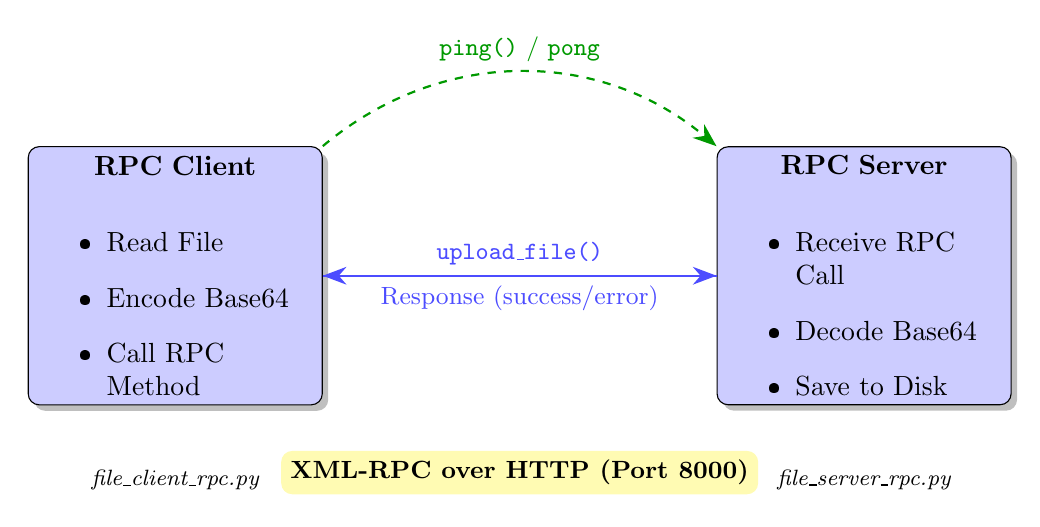
\begin{tikzpicture}[node distance=3cm,
    box/.style={rectangle, draw, fill=blue!20, text width=3.5cm, align=center, minimum height=2.5cm, rounded corners, drop shadow},
    arrow/.style={-{Stealth[length=3mm]}, thick},
    label/.style={font=\small}]
    
    % Client box
    \node[box] (client) {\textbf{RPC Client}\\
        \vspace{0.2cm}
        \begin{itemize}
            \item Read File
            \item Encode Base64
            \item Call RPC Method
        \end{itemize}};
    
    % Server box
    \node[box, right=5cm of client] (server) {\textbf{RPC Server}\\
        \vspace{0.2cm}
        \begin{itemize}
            \item Receive RPC Call
            \item Decode Base64
            \item Save to Disk
        \end{itemize}};
    
    % Main communication arrow
    \draw[arrow, blue!70] (client.east) -- node[above, label] {\texttt{upload\_file()}} (server.west);
    \draw[arrow, blue!70] (server.west) -- node[below, label] {Response (success/error)} (client.east);
    
    % Ping connection (curved)
    \draw[arrow, green!60!black, dashed] (client.north east) to[bend left=40] node[above, label, green!60!black] {\texttt{ping()} / \texttt{pong}} (server.north west);
    
    % Protocol label
    \node[below=0.7cm of client, font=\footnotesize\itshape] {file\_client\_rpc.py};
    \node[below=0.7cm of server, font=\footnotesize\itshape] {file\_server\_rpc.py};
    
    % Connection line label (moved down to avoid overlap)
    \node[fill=yellow!30, rounded corners, font=\small\bfseries] at ($(client.east)!0.5!(server.west) + (0,-2.5)$) {XML-RPC over HTTP (Port 8000)};
    
\end{tikzpicture}
\caption{RPC File Transfer System Architecture}
\label{fig:architecture}
\end{figure}

\subsection{Design Principles}

\begin{itemize}
    \item \textbf{Simplicity}: XML-RPC provides automatic serialization and deserialization, eliminating the need for manual protocol implementation.
    \item \textbf{Transparency}: Remote method calls appear as local function calls to the developer.
    \item \textbf{HTTP-based}: Uses HTTP as the transport protocol, making it firewall-friendly.
    \item \textbf{Base64 Encoding}: Binary file data is encoded to Base64 for safe transmission over XML-RPC.
\end{itemize}

\subsection{RPC Methods}

The server exposes the following RPC methods:

\begin{enumerate}
    \item \texttt{upload\_file(filename, file\_data\_base64)}: Receives and saves a file to the server
    \item \texttt{ping()}: Tests server connectivity and returns ``pong''
    \item \texttt{get\_server\_info()}: Returns server information including name, version, and configuration
\end{enumerate}

\section{System Organization}

\subsection{Component Structure}

The system is organized into clear client and server components, as shown in Figure \ref{fig:organization}.

\begin{figure}[H]
\centering
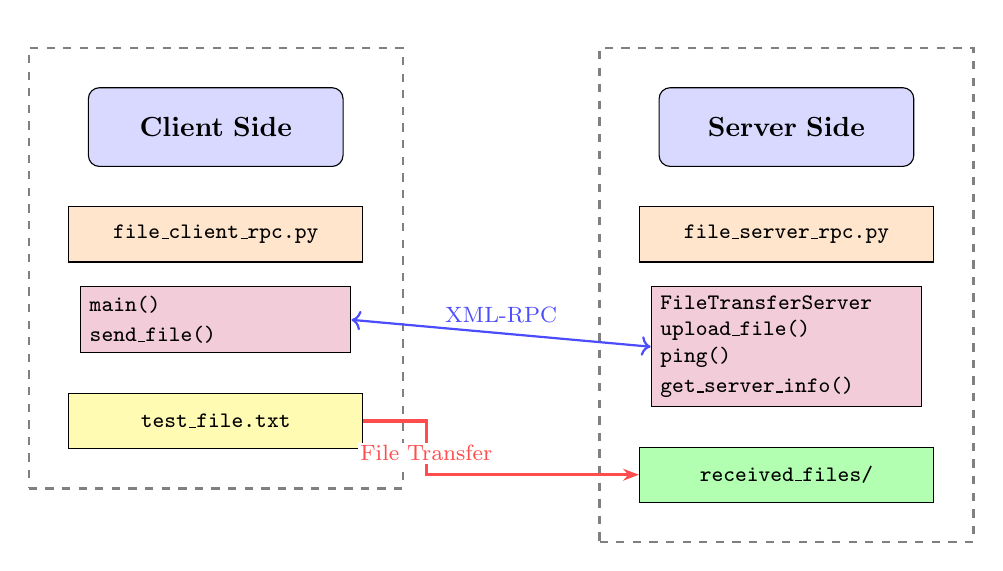
\begin{tikzpicture}[node distance=2cm,
    component/.style={rectangle, draw, fill=green!20, text width=3cm, align=center, minimum height=1cm, rounded corners},
    file/.style={rectangle, draw, fill=orange!20, text width=3.5cm, align=center, minimum height=0.7cm, font=\footnotesize},
    class/.style={rectangle, draw, fill=purple!20, text width=3.2cm, align=left, minimum height=0.8cm, font=\small},
    container/.style={rectangle, draw=black!50, dashed, thick, inner sep=0.5cm},
    arrow/.style={-{Stealth[length=2mm]}, thick}]
    
    % Client Side Container
    \node[component, fill=blue!15] (client_title) {\textbf{Client Side}};
    \node[file, below=0.5cm of client_title] (client_file) {\texttt{file\_client\_rpc.py}};
    \node[class, below=0.3cm of client_file] (client_funcs) {\footnotesize
        \texttt{main()}\\
        \texttt{send\_file()}};
    \node[file, below=0.5cm of client_funcs, fill=yellow!30] (test_file) {\texttt{test\_file.txt}};
    
    \node[container, fit=(client_title)(client_file)(client_funcs)(test_file), label=above:] (client_box) {};
    
    % Server Side Container
    \node[component, fill=blue!15, right=4cm of client_title] (server_title) {\textbf{Server Side}};
    \node[file, below=0.5cm of server_title] (server_file) {\texttt{file\_server\_rpc.py}};
    \node[class, below=0.3cm of server_file] (server_class) {\footnotesize
        \texttt{FileTransferServer}\\
        \texttt{upload\_file()}\\
        \texttt{ping()}\\
        \texttt{get\_server\_info()}};
    \node[file, below=0.5cm of server_class, fill=green!30] (received_dir) {\texttt{received\_files/}};
    
    \node[container, fit=(server_title)(server_file)(server_class)(received_dir), label=above:] (server_box) {};
    
    % Data flow arrows
    \draw[arrow, red!70, very thick] (test_file.east) -- ++(0.8,0) |- node[pos=0.3, font=\footnotesize, fill=white, inner sep=1pt] {File Transfer} (received_dir.west);
    
    % RPC communication
    \draw[arrow, blue!70, thick, <->] (client_funcs.east) -- node[above, font=\footnotesize] {XML-RPC} (server_class.west);
    
\end{tikzpicture}
\caption{System Organization and Component Structure}
\label{fig:organization}
\end{figure}


\subsection{Key Components}

\begin{itemize}
    \item \textbf{Server Component}: 
        \begin{itemize}
            \item \texttt{FileTransferServer} class encapsulates RPC methods
            \item Handles file reception, decoding, and storage
            \item Provides introspection capabilities
        \end{itemize}
    
    \item \textbf{Client Component}:
        \begin{itemize}
            \item \texttt{send\_file()} function manages file transmission
            \item Handles Base64 encoding and RPC method invocation
            \item Provides user-friendly command-line interface
        \end{itemize}
\end{itemize}

\section{Implementation Details}

\subsection{Server Implementation}

The server uses Python's \texttt{SimpleXMLRPCServer} to expose RPC methods. Key implementation snippet:

\begin{lstlisting}[caption=Server RPC Method Implementation]
def upload_file(self, filename, file_data_base64):
    """
    RPC method to receive and save a file
    """
    try:
        # Decode base64 data
        file_data = base64.b64decode(file_data_base64)
        
        # Create filepath
        filepath = os.path.join(self.received_dir, filename)
        
        # Write file
        with open(filepath, 'wb') as f:
            f.write(file_data)
        
        filesize = len(file_data)
        
        return {
            'status': 'success',
            'message': f'File {filename} uploaded successfully',
            'size': filesize,
            'path': filepath
        }
    except Exception as e:
        return {
            'status': 'error',
            'message': f'Error uploading file: {str(e)}'
        }
\end{lstlisting}

\subsection{Client Implementation}

The client creates a proxy object to call remote methods:

\begin{lstlisting}[caption=Client RPC Invocation]
def send_file(filename, host='127.0.0.1', port=8000):
    """Send file to RPC server"""
    # Create RPC client proxy
    server_url = f"http://{host}:{port}"
    proxy = xmlrpc.client.ServerProxy(server_url)
    
    # Test connection
    response = proxy.ping()
    
    # Read and encode file
    with open(filename, 'rb') as f:
        file_data = f.read()
    
    file_data_base64 = base64.b64encode(file_data).decode('utf-8')
    
    # Call RPC method
    result = proxy.upload_file(basename, file_data_base64)
    
    return result['status'] == 'success'
\end{lstlisting}

\subsection{Data Flow}

The file transfer process follows these steps:

\begin{enumerate}
    \item Client reads the file from disk into memory
    \item File data is encoded to Base64 string
    \item Client invokes \texttt{upload\_file()} RPC method with filename and encoded data
    \item XML-RPC library serializes the call to XML and sends via HTTP
    \item Server receives HTTP request and deserializes XML to Python objects
    \item Server decodes Base64 data back to binary
    \item Server writes binary data to disk in \texttt{received\_files/} directory
    \item Server returns success/error response
    \item Client receives response and displays result
\end{enumerate}

\section{Comparison with TCP Implementation}

\begin{table}[H]
\centering
\begin{tabular}{|l|p{5cm}|p{5cm}|}
\hline
\textbf{Aspect} & \textbf{TCP Implementation} & \textbf{RPC Implementation} \\ \hline
Protocol & Raw TCP sockets & XML-RPC over HTTP \\ \hline
Communication & Manual protocol with struct packing & Remote procedure calls \\ \hline
Complexity & Higher (manual handling) & Lower (abstracted) \\ \hline
Code Length & ~200 lines & ~180 lines \\ \hline
Error Handling & Manual socket error handling & Built-in RPC error handling \\ \hline
Data Encoding & Binary with struct.pack & Base64 encoding \\ \hline
\end{tabular}
\caption{Comparison between TCP and RPC implementations}
\end{table}


\section{Testing and Results}

\subsection{Test Environment}
\begin{itemize}
    \item Operating System: Windows 10/11
    \item Python Version: 3.x
    \item Server: localhost:8000
    \item Test File: test\_file.txt (292 bytes)
\end{itemize}

\subsection{Test Results}

\begin{enumerate}
    \item \textbf{Server Startup}: Successfully starts and listens on port 8000
    \item \textbf{Client Connection}: Successfully connects and pings server
    \item \textbf{File Transfer}: File transferred completely and correctly
    \item \textbf{File Integrity}: MD5 checksum matches for original and received files
    \item \textbf{Error Handling}: Proper error messages for non-existent files and connection failures
\end{enumerate}

\section{Conclusion}

The RPC-based file transfer system successfully demonstrates the advantages of using remote procedure calls over raw socket programming. The implementation is cleaner, more maintainable, and easier to understand while providing the same functionality as the TCP version. The use of XML-RPC abstracts away the low-level network details, allowing developers to focus on the business logic rather than protocol implementation.

\subsection{Advantages of RPC Approach}
\begin{itemize}
    \item Simplified code structure
    \item Automatic serialization/deserialization
    \item Built-in error handling
    \item Better abstraction of network communication
\end{itemize}

\subsection{Future Improvements}
\begin{itemize}
    \item Implement chunked transfer for large files
    \item Add authentication and encryption
    \item Support for multiple concurrent clients
    \item Progress callback for real-time transfer updates
\end{itemize}

\end{document}
